\documentclass{article}

% Preamble with required packages
\usepackage{amsmath, amssymb, amsthm}
\usepackage{algorithm}
\usepackage{algpseudocode}
\usepackage[cache=false]{minted}
\usepackage{fvextra}
\setminted{breaklines=true}
\usepackage{listings}
\usepackage{float}
\usepackage{tabularx}
\usepackage{geometry}
\usepackage{xcolor}
\usepackage{colortbl}
\usepackage{hyperref}
\usepackage{graphicx}
\usepackage{physics} % For \ket{} command
\usepackage{color}
\usepackage{booktabs}

\definecolor{codegreen}{rgb}{0,0.6,0}
\definecolor{codegray}{rgb}{0.5,0.5,0.5}
\definecolor{codepurple}{rgb}{0.58,0,0.82}
\definecolor{backcolour}{rgb}{0.95,0.95,0.92}

\lstdefinestyle{mystyle}{
    backgroundcolor=\color{backcolour},   
    commentstyle=\color{codegreen},
    keywordstyle=\color{magenta},
    numberstyle=\tiny\color{codegray},
    stringstyle=\color{codepurple},
    basicstyle=\ttfamily\small,
    breakatwhitespace=false,         
    breaklines=true,                 
    captionpos=b,                    
    keepspaces=true,                 
    numbers=left,                    
    numbersep=5pt,                  
    showspaces=false,                
    showstringspaces=false,
    showtabs=false,                  
    tabsize=2
}

\lstset{
    language=python,
    style=mystyle
}
\usepackage{hyperref}
\hypersetup{
    colorlinks=true,
    linkcolor=blue!70!black,
    filecolor=blue!70!black,
    urlcolor=blue!70!black,
    citecolor=blue!70!black,
    pdftitle={Breaking RSA with Quantum Fourier Transforms},
    pdfauthor={Group Assignment 1},
    pdfborder={0 0 0},
}

% Add this to your preamble
\usepackage{tcolorbox}
\usepackage{xcolor}

% Define alert box styles
\newtcolorbox{infobox}[1][]{
    colback=blue!5!white,
    colframe=blue!75!black,
    fonttitle=\bfseries,
    title={Information},
    #1
}

\newtcolorbox{warningbox}[1][]{
    colback=yellow!10!white,
    colframe=yellow!75!black,
    fonttitle=\bfseries,
    title={Warning},
    #1
}

\newtcolorbox{successbox}[1][]{
    colback=green!5!white,
    colframe=green!75!black,
    fonttitle=\bfseries,
    title={Success},
    #1
}

\newtcolorbox{errorbox}[1][]{
    colback=red!5!white,
    colframe=red!75!black,
    fonttitle=\bfseries,
    title={Error},
    #1
}

\newtcolorbox{notebox}[1][]{
    colback=gray!5!white,
    colframe=gray!75!black,
    fonttitle=\bfseries,
    title={Note},
    #1
}

\newtcolorbox{definitionbox}[1][]{
    colback=purple!5!white,
    colframe=purple!75!black,
    fonttitle=\bfseries,
    title={Definition},
    #1
}



% If you don't want to use the physics package, uncomment this line:
% \newcommand{\ket}[1]{|#1\rangle}

% Define theorem-like environments
\newtheorem{definition}{Definition}
\newtheorem{example}{Example}

% Page layout
\geometry{a4paper, margin=1in}
\setlength{\parindent}{0pt}

\title{\Huge\textsc{Breaking RSA \\ with \\ Quantum Fourier Transforms}}
\author{
    \Large\textsc{\vspace{2cm} IC121 Mechanics of Particles and Waves}\\[2ex]
        \LARGE\textsc{Group Assignment 1}\vspace{0.5cm}\\
        \Large{Group Number: 19}\\[2cm]
        \textbf{\Large Group Members}\vspace{0.5cm}\\[1ex]
        \begin{tabular}{r|l} 
            \hline \hline
            \textsc{Name} & \textsc{Roll No.} \\ \hline 
            Abhishek \textsc{Mantri}        & B23060 \\ 
            Harshit \textsc{Jain}           & B23132 \\
            Arani \textsc{Ghosh}            & B23119 \\
            Jigar \textsc{Fufal}            & B24244 \\
            Arka \textsc{Mukhopadhay}       & B23120 \\
            Ojas \textsc{More}              & B24263 \\
            Parth \textsc{Gawande}          & B24266 \\ 
            \hline \hline
        \end{tabular}
        \vspace{5cm}
}
\date{\today}

\begin{document}

\maketitle
\newpage
\tableofcontents
\newpage

\section{What is RSA?}

\begin{infobox}[title=RSA Overview]
    RSA is an asymmetric cryptography algorithm widely used for secure data transmission. Asymmetric, or public-key cryptography, uses two different keys: a public key for encryption and a private key for decryption. The public key can be freely distributed, while the private key must be kept secret.
\end{infobox}

\subsection{RSA Key Generation}

\begin{algorithm}
    \caption{RSA Key Generation}
    \begin{algorithmic}[1]
        \State Choose two distinct large prime numbers, $p$ and $q$.
        \State Compute the modulus $n = p \times q$. This $n$ is part of both the public and private keys.
        \State Calculate Euler's totient function: $\varphi(n) = (p - 1)(q - 1)$.
        \State Choose an integer $e$ such that $1 < e < \varphi(n)$ and $\gcd(e, \varphi(n)) = 1$. This $e$ is the public exponent.
        \State Compute an integer $d$ such that $(d \times e) \equiv 1 \pmod{\varphi(n)}$. This $d$ is the private exponent.
    \end{algorithmic}
\end{algorithm}

The public key is $(n, e)$. The private key is $(n, d)$. The primes $p$ and $q$, and $\varphi(n)$ should also be kept secret.

\subsection{Encryption and Decryption}

\textbf{Encryption:} To encrypt a message $m$ (with $0 \leq m < n$), compute the ciphertext $c$ as:
\[
    c \equiv m^e \pmod{n}
\]

\textbf{Decryption:} To decrypt $c$, compute:
\[
    m \equiv c^d \pmod{n}
\]

\section{Weaknesses of RSA}

\begin{warningbox}[title=Security Vulnerabilities]
    Despite its widespread use, RSA has several vulnerabilities:

    \begin{itemize}
        \item \textbf{Poor Choice of Primes:} If the primes $p$ and $q$ are chosen poorly, factorization becomes easier. For example, if $p$ and $q$ are too close to each other (e.g., $|p-q| \ll \sqrt{n}$), Fermat's factorization method becomes efficient. Similarly, if one prime is significantly smaller than the other, Elliptic Curve Factorization (ECF) can effectively factor the modulus.

        \item \textbf{Small Modulus:} If the modulus $n$ is too small, it can be factored easily. Secure RSA uses moduli of at least 2048 bits.

        \item \textbf{Low Public Exponent:} A small exponent $e$ (e.g., 3) may speed up encryption, but if used improperly (e.g., encrypting the same message with the same $e$ and different moduli), it can allow recovery of the plaintext using techniques like the Chinese Remainder Theorem. Also, if $m^e < n$, the ciphertext $c = m^e$ leaks $m$ directly.

        \item \textbf{Weak Random Number Generation:} Poor or predictable generation of primes $p$ and $q$ can allow attackers to factor $n$ and break the encryption.

        \item \textbf{Side-Channel Attacks:} These exploit physical characteristics like timing or power usage during encryption/decryption to gain insights into the private key.

        \item \textbf{Advanced Factoring Algorithms:} Techniques such as the General Number Field Sieve (GNFS) continue to improve and pose a threat to RSA's long-term security.

        \item \textbf{Quantum Threats:} Algorithms like Shor's, running on quantum computers, can factor large integers efficiently, potentially rendering RSA obsolete.
    \end{itemize}
\end{warningbox}

\section{Fermat's Factorization for Close Primes}

\begin{definitionbox}[title=Fermat's Factorization]
    If $n = a^2 - b^2 = (a - b)(a + b)$, then $p = a - b$ and $q = a + b$ are factors of $n$.
\end{definitionbox}

Fermat's factorization method exploits a fundamental algebraic identity: the difference of squares. When an RSA modulus $n = pq$ can be expressed as $a^2 - b^2$ for some integers $a$ and $b$, we can immediately factor $n$ as $(a-b)(a+b)$.
\newline

\begin{algorithm}
    \caption{Fermat's Factorization Method}
    \begin{algorithmic}[1]
        \State Start with $a = \lceil\sqrt{n}\rceil$
        \State Calculate $b^2 = a^2 - n$
        \State Check if $b^2$ is a perfect square
        \State If yes, compute $p = a - b$ and $q = a + b$
        \State If no, increment $a$ and repeat from step 2
    \end{algorithmic}
\end{algorithm}

\textbf{Exploiting Close Primes:} If $p$ and $q$ are close to each other, this method becomes highly efficient. When $p \approx q$, their arithmetic mean $\frac{p+q}{2}$ is approximately $\sqrt{n}$, making $a \approx \sqrt{n}$. The search for $a$ typically requires very few iterations, making the factorization trivial.

This vulnerability highlights why proper RSA implementations should use primes that are sufficiently far apart. Modern standards recommend that $|p-q| > 2^{(n/2-100)}$ where $n$ is the bit length of the modulus.

\begin{example}
    Suppose $n = 851$. Then $\sqrt{851} \approx 29.17$.

    Try $x = 30$: $30^2 - 851 = 900 - 851 = 49 = 7^2$.

    So $x = 30$, $y = 7$, $p = 30 - 7 = 23$, $q = 30 + 7 = 37$.

    Indeed, $23 \times 37 = 851$.
\end{example}

\lstinputlisting[caption=SageMath Implementation of Fermat's Factorization Theorem]{../sims/fermats_sage.sage}

\begin{notebox}[title=Implementation Note]
    This implementation demonstrates Fermat's factorization method, which is particularly effective when the prime factors are close together. The algorithm starts with the ceiling of the square root of the modulus and increments until it finds a value that makes $a^2 - n$ a perfect square, allowing for easy factorization.
\end{notebox}

\section{Elliptic Curve Factorization (ECF)}

\begin{definitionbox}[title=ECF Definition]
    Elliptic Curve Factorization (ECF), developed by Hendrik Lenstra, is a probabilistic algorithm whose running time primarily depends on the size of the smallest prime factor of $n$, rather than the size of $n$ itself.
\end{definitionbox}

ECF operates by performing computations on randomly chosen elliptic curves over finite fields. Unlike Fermat's factorization method, which is specifically efficient when factors are close together, ECF is more versatile and effective when $n$ has relatively small prime factors, regardless of their proximity.

\subsection*{How ECF Works}

The Elliptic Curve Factorization method works through the following process:

\begin{algorithm}
    \caption{Elliptic Curve Factorization Method}
    \begin{algorithmic}[1]
        \State Choose a random elliptic curve $E$ over the ring $\mathbb{Z}_n$
        \State Select a random point $P$ on the curve $E$
        \State Attempt to perform scalar multiplication $kP$ for a large integer $k$
        \State During computation, if an inverse modulo $n$ cannot be computed (i.e., $\gcd(\text{denominator}, n) \neq 1$)
        \State Extract the non-trivial factor of $n$ as $\gcd(\text{denominator}, n)$
        \State If no factor is found, repeat with a different curve and/or point
    \end{algorithmic}
\end{algorithm}

The key insight is that a failure in modular inversion during point arithmetic reveals a factor of the modulus. This makes ECF particularly effective when $n$ has a relatively small prime factor.

\subsection*{When is ECF a Viable Attack on RSA?}

The Elliptic Curve Factorization method (ECF), or Elliptic Curve Method (ECM), is effective when one of the RSA prime factors is relatively small—typically under 200-230 bits. Unlike Fermat's attack, which exploits closeness between \( p \) and \( q \), ECF focuses on the \emph{absolute size} of the smaller factor.

\begin{itemize}
    \item \textbf{Best suited for small primes:} If one of the primes is small, ECF can factor the modulus efficiently, regardless of how close \( p \) and \( q \) are.
    \item \textbf{More general than Fermat's method:} As discussed earlier, Fermat's method works best when \( p \approx q \). ECF does not rely on this closeness and remains effective over a wider range of factor pairs.
    \item \textbf{Ineffective for strong keys:} When both \( p \) and \( q \) are large (e.g., 1024 bits each), ECF becomes infeasible.
\end{itemize}

\noindent Thus, ECF is particularly useful for detecting weak RSA keys where one prime is significantly smaller, even if \( p \) and \( q \) are not close.


\section{Fourier Transform}

\begin{definitionbox}[title=Fourier Transform]
    The Fourier Transform of a function $f(t)$ is a mathematical transformation that decomposes the function into its constituent frequencies:
    \[
        F(\omega) = \int_{-\infty}^{\infty} f(t) e^{-j\omega t} \, dt
    \]
    where $\omega$ represents angular frequency, $j$ is the imaginary unit $\sqrt{-1}$, and $e^{-j\omega t} = \cos(\omega t) - j\sin(\omega t)$ are the complex exponential basis functions.
\end{definitionbox}

\begin{figure}[!ht]
    \centering
    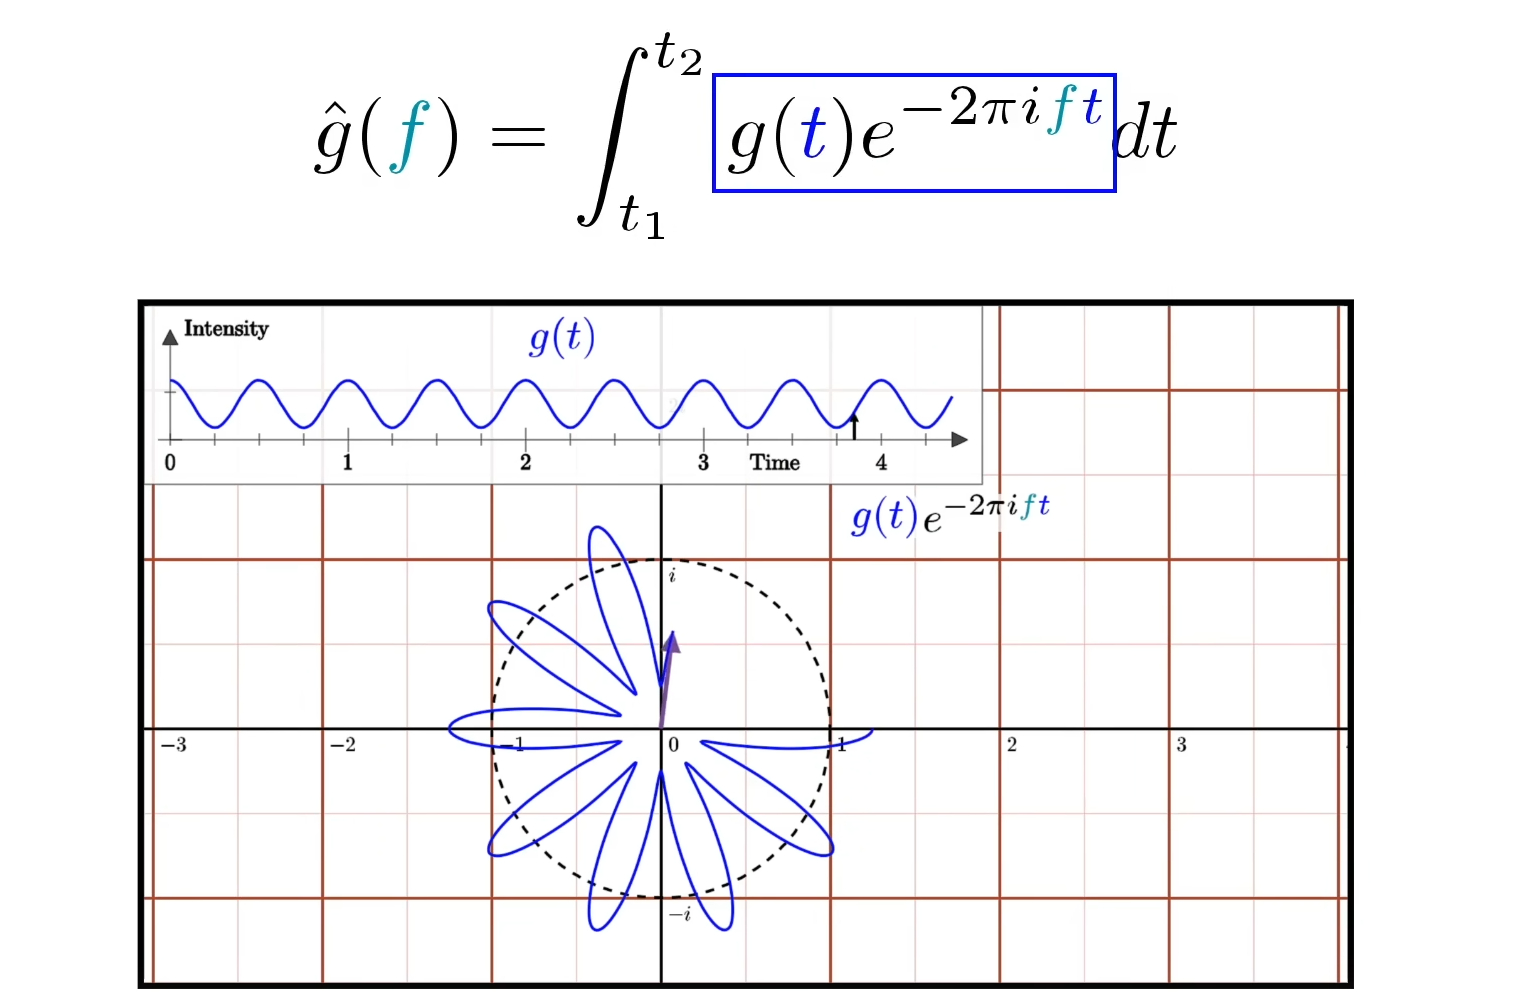
\includegraphics[width=\textwidth]{./pics/convolv.png}
    \caption{Fourier Transform}
    \label{fig:fourier_transform}
\end{figure}

\begin{figure}[!ht]
    \centering
    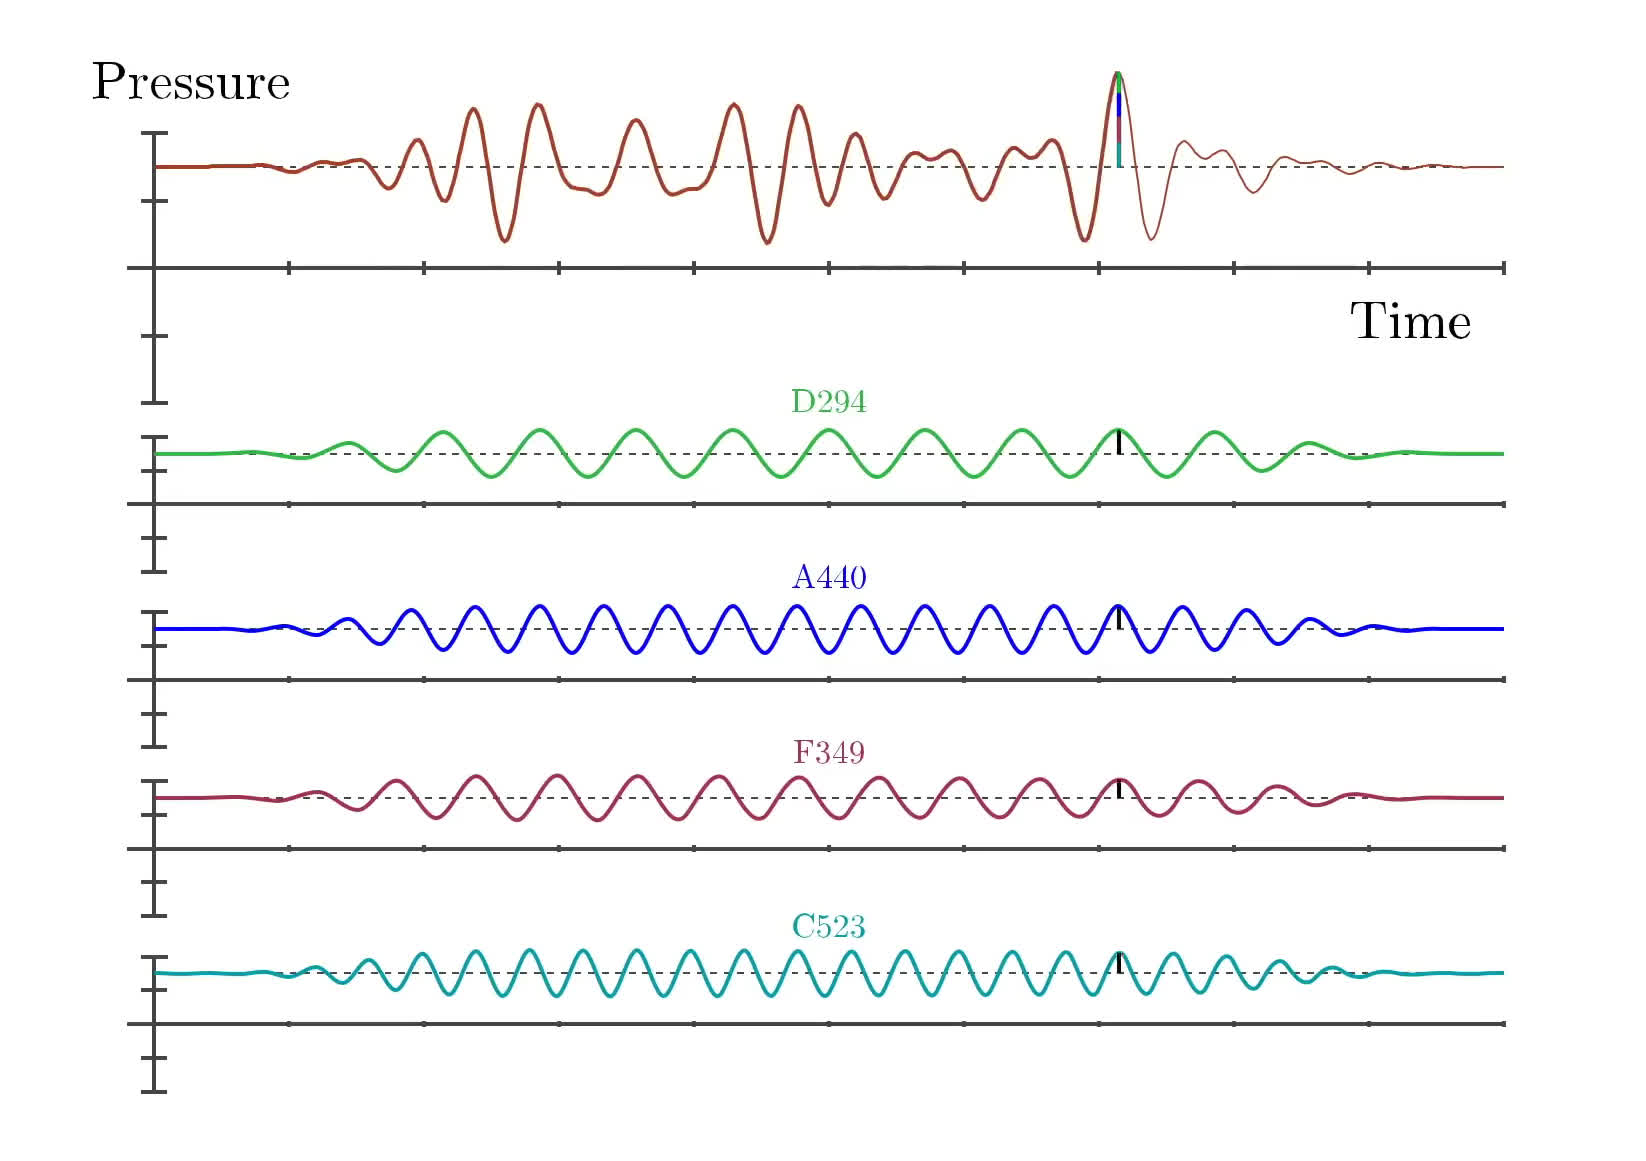
\includegraphics[width=\textwidth]{./pics/decomp.png}
    \caption{Signal Decomposition}
    \label{fig:signal_decomp}
\end{figure}


The inverse Fourier Transform allows reconstruction of the original signal from its frequency components:
\[
    f(t) = \frac{1}{2\pi} \int_{-\infty}^{\infty} F(\omega) e^{j\omega t} \, d\omega
\]

\begin{figure}[!ht]
    \centering
    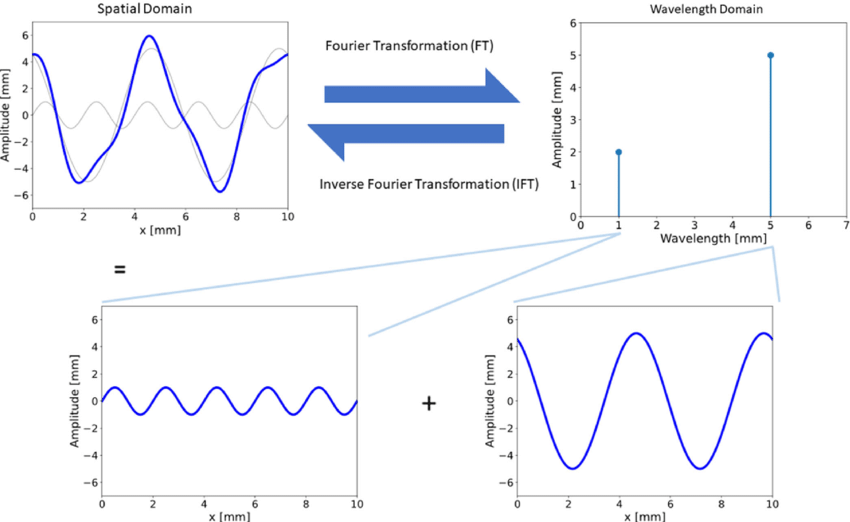
\includegraphics[width=\textwidth]{./pics/inverse-fourier-transform.png}
    \caption{Inverse Fourier Transform}
    \label{fig:inv_fourier_transform}
\end{figure}

For practical applications with discrete signals (like digital cryptographic data), the Discrete Fourier Transform (DFT) is used:
\[
    X_k = \sum_{n=0}^{N-1} x_n e^{-j \frac{2\pi}{N} kn}, \quad k = 0,1,\ldots,N-1
\]
where:
\begin{itemize}
    \item $x_n$ is the $n$-th sample of the discrete signal of length $N$
    \item $X_k$ is the $k$-th frequency component
\end{itemize}

The DFT is computationally expensive, requiring $\mathcal{O}(N^2)$ operations. The Fast Fourier Transform (FFT) algorithm reduces this to $\mathcal{O}(N \log N)$, making it feasible for large datasets.

\lstinputlisting[caption=Basic Implementation of Fast Fourier Transform using NumPy]{../sims/fourier_basic_implementation.py}


\section{Fourier Transforms and Wrapped Waveforms}

The Fourier transform can be intuitively understood through the concept of "wrapped waveforms" and their centers of gravity, providing a geometric interpretation of frequency analysis.

\subsection{The Wrapping Process}

Imagine taking a time-domain signal $f(t)$ and wrapping it around the unit circle in the complex plane:

\begin{itemize}
    \item For a specific frequency $\omega$, each time point $t$ corresponds to a position $e^{j\omega t}$ on the unit circle.
    \item The value of $f(t)$ at each point determines the "weight" placed at that position on the circle.
    \item As we integrate over all time, we effectively distribute weights around the circle according to the signal's values.
\end{itemize}

\subsection{Center of Gravity Interpretation}

The Fourier transform $F(\omega)$ at frequency $\omega$ can be interpreted as the center of gravity (or center of mass) of this wrapped waveform:

\[
    F(\omega) = \int_{-\infty}^{\infty} f(t) e^{-j\omega t} \, dt
\]

When the frequency $\omega$ matches a significant frequency component in the signal:
\begin{itemize}
    \item The signal wraps in a way that aligns coherently around the circle
    \item Weights accumulate at specific positions rather than canceling out
    \item The center of gravity moves away from the origin, resulting in a larger magnitude $|F(\omega)|$
\end{itemize}

When $\omega$ doesn't match a frequency present in the signal:
\begin{itemize}
    \item The signal wraps incoherently, distributing weights more uniformly around the circle
    \item These uniform weights tend to cancel each other out
    \item The center of gravity remains close to the origin, resulting in a smaller magnitude $|F(\omega)|$
\end{itemize}

\subsection{Mathematical Expression}

If we express the complex exponential in terms of sines and cosines:
\[
    F(\omega) = \int_{-\infty}^{\infty} f(t) \cos(\omega t) \, dt - j\int_{-\infty}^{\infty} f(t) \sin(\omega t) \, dt
\]

The real part represents the projection of the center of gravity onto the real axis, while the imaginary part represents the projection onto the imaginary axis.

\begin{figure}[p]
    \centering
    \rotatebox{90}{
        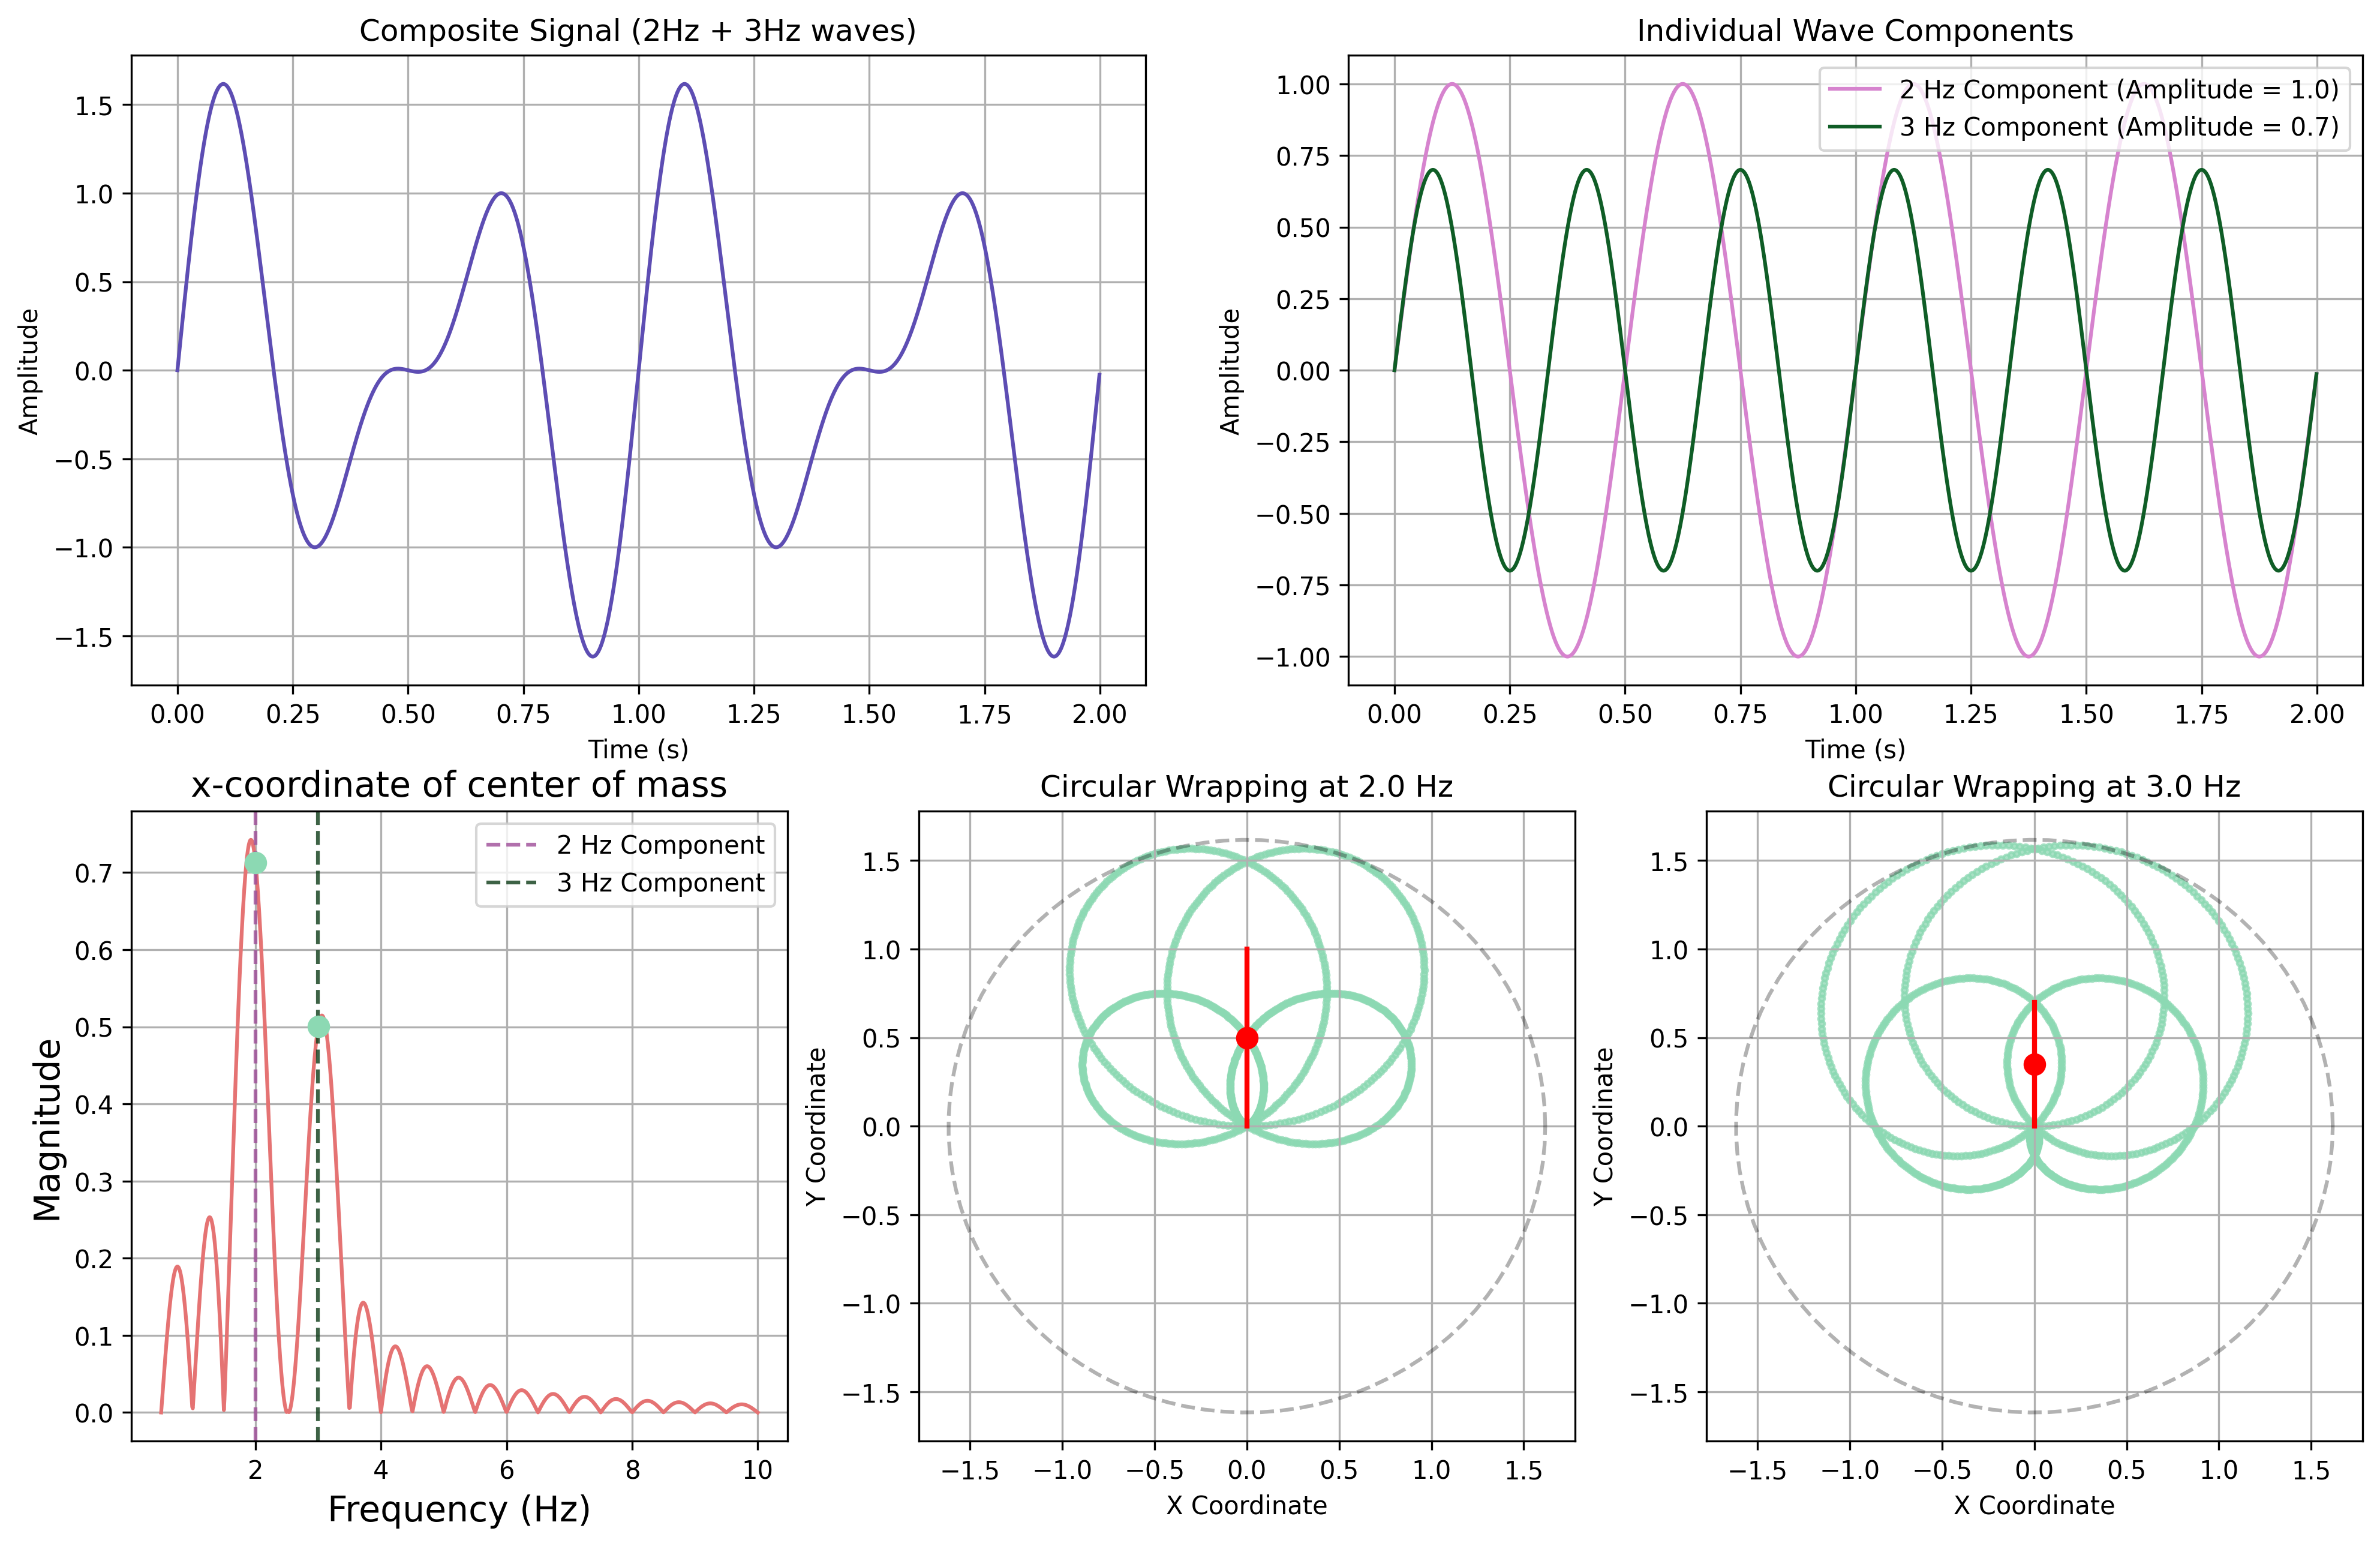
\includegraphics[width=0.95\textheight]{./pics/complete_fourier.png}
    }
    \caption{Wrapping and its relation to Fourier Transform}
    \label{fig:complete_fourier}
\end{figure}


\section{Introduction to Quantum Computing}

\begin{infobox}[title=Quantum Computing Fundamentals]
    Quantum computing is an emerging paradigm that leverages the principles of quantum mechanics to process information in fundamentally new ways. Unlike classical computing, which relies on bits to represent data as either 0 or 1, quantum computing introduces the concept of qubits---quantum bits---that enable powerful computational capabilities through unique quantum phenomena.
\end{infobox}

\subsection{Qubits: The Quantum Information Unit}

\begin{definitionbox}[title=Qubit]
    A qubit (just a fancy short for quantum bit) can exist not just in the classical states $\ket{0}$ or $\ket{1}$, but in a superposition of both:
    \[
        \ket{\psi} = \alpha \ket{0} + \beta \ket{1}
    \]
    Here, $\alpha$ and $\beta$ are complex numbers called \emph{probability amplitudes}, and they determine the likelihood of the qubit being measured in state $\ket{0}$ or $\ket{1}$.
\end{definitionbox}

Superposition is essentially the ability of a qubit to simultaneously represent a linear combination of both basis states, $\ket{0}$ and $\ket{1}$. The probabilities of measuring the qubit in each state are given by the squared magnitudes of the amplitudes:
\[
    |\alpha|^2 + |\beta|^2 = 1
\]
This equation ensures that the total probability of all possible outcomes is 1. The state $\ket{\psi}$ is called the \emph{quantum state}, a vector in a 2-dimensional complex Hilbert space. This state captures all information about how a qubit behaves under observation or interaction.

\subsection{Quantum Gates: Manipulating Qubit States}
Just as classical computers use logic gates (like AND, OR, NOT) to process bits, quantum computers use \emph{quantum gates} to manipulate qubits.

Quantum gates are mathematical operations that change the state of a qubit. They act on the qubit's quantum state vector in its complex vector space, and are typically represented by unitary matrices. These operations are reversible, unlike many classical gates.

For example:
\begin{itemize}
    \item The \textbf{Hadamard gate (H)} creates superposition by transforming a qubit from a definite state ($\ket{0}$ or $\ket{1}$) into an equal combination of both.
    \item The \textbf{Pauli-X gate} is the quantum equivalent of a classical NOT gate; it flips $\ket{0}$ to $\ket{1}$ and vice versa.
\end{itemize}

Gates are the tools that let us harness and direct the quantum properties of qubits, enabling computation. Without gates, qubits just sit there in superposition. With gates, we build quantum circuits that perform real tasks—leading up to the final step of measurement, where the quantum result is extracted.

\subsection{Analogy: Bits vs Qubits}
A simple analogy illustrates the distinction:

\begin{itemize}
    \item A classical bit is like a coin resting on a table---it's either heads (0) or tails (1).
    \item A qubit in superposition is like a spinning coin in mid-air---it's in a genuine mixture of heads and tails until it lands (i.e., until it's measured).
\end{itemize}

This analogy captures the essence of quantum uncertainty and parallelism.

\subsection{Measurement: From Superposition to Classical State}
When a qubit is measured, it collapses from its superposed state into one of the two classical states---$\ket{0}$ or $\ket{1}$. The outcome is random, governed by the probabilities $|\alpha|^2$ and $|\beta|^2$. After measurement, the qubit loses its superposition and remains in the resulting classical state.

The process of measurement is inherently destructive to superposition, and its exact implementation depends on the physical realization of the qubit. For example:

\begin{itemize}
    \item In the \textbf{Superconducting Qubits (used by IBM)}: Measurement is performed using microwave pulses and a resonator that detects the resulting quantum state.
\end{itemize}


\section{Quantum Fourier Transform (QFT)}

\begin{infobox}[title=QFT Overview]
    The Quantum Fourier Transform (QFT) is a fundamental operation in quantum computing, serving as the quantum counterpart to the classical Discrete Fourier Transform (DFT).

    In classical computing, the DFT converts a sequence of complex numbers into another sequence that represents the frequency components of the original sequence. Similarly, the QFT operates on the amplitudes of a quantum state, transforming them into a superposition of states with different amplitudes.
\end{infobox}

The QFT operates on an $n$-qubit quantum state $\ket{x}$, transforming it into a superposition of states weighted by complex exponential factors:
\[
    \text{QFT}(\ket{x}) = \frac{1}{\sqrt{N}} \sum_{k=0}^{N-1} e^{2\pi i xk / N} \ket{k}, \quad N = 2^n
\]
This transformation is unitary and reversible, preserving the total probability of the quantum system.

\subsection{Implementing the QFT in Quantum Circuits}

The QFT can be efficiently implemented using a sequence of quantum gates:
\begin{itemize}
    \item \textbf{Hadamard Gates}: Applied to individual qubits to create superpositions.
    \item \textbf{Controlled Phase Shift Gates}: Introduce relative phases between qubits based on their states.
    \item \textbf{Swap Gates}: Reverse the order of qubits to obtain the correct output.
\end{itemize}

This implementation requires $\mathcal{O}(n^2)$ quantum gates, making it exponentially faster than the classical Fast Fourier Transform (FFT) for large datasets.

\subsection{Connection to Wrapping Intuition}

This wrapping process provides an intuitive basis for understanding the Quantum Fourier Transform. In quantum computing, the QFT essentially performs this wrapping operation on quantum amplitudes rather than classical signal values. The phase relationships between different components of a quantum state play a role analogous to the weights distributed around the unit circle.

When a quantum state has periodic structure, the QFT transforms this into a state with amplitudes concentrated at specific frequencies—just as a periodic classical signal produces peaks in its Fourier spectrum. This property makes the QFT particularly useful for detecting periodicity in quantum algorithms like Shor's, which is crucial for factoring integers.

\subsection{Applications}

The QFT is instrumental in several quantum algorithms:

\begin{itemize}
    \item \textbf{Shor's Algorithm}: Utilizes the QFT for efficient integer factorization, which has implications for cryptography.
    \item \textbf{Quantum Phase Estimation}: Employs the QFT to estimate the phase (eigenvalues) of unitary operators, a critical component in various quantum algorithms.
\end{itemize}

\section{Shor's Algorithm}

\begin{successbox}[title=Quantum Advantage]
    Shor's Algorithm is a groundbreaking quantum algorithm developed by mathematician Peter Shor in 1994. It efficiently factors large integers, a task that is computationally intensive for classical computers. This capability poses significant implications for cryptography, particularly for encryption methods like RSA that rely on the difficulty of prime factorization.
\end{successbox}

\subsection{How Shor's Algorithm Works}

The algorithm comprises both classical and quantum components:

\begin{algorithm}[H]
    \caption{Shor's Algorithm for Integer Factorization}
    \begin{algorithmic}[1]
        \State \textbf{Classical Preprocessing:}
        \State \hspace{0.5cm} Select a random integer $a$ such that $1 < a < N$ and $\gcd(a, N) = 1$
        \State \hspace{0.5cm} If $\gcd(a, N) \neq 1$, a nontrivial factor is found

        \State \textbf{Quantum Order Finding:}
        \State \hspace{0.5cm} Utilize a quantum computer to find the period $r$ of the function $f(x) = a^x \mod N$
        \State \hspace{0.5cm} This step employs quantum parallelism and the QFT to determine $r$ efficiently

        \State \textbf{Classical Postprocessing:}
        \State \hspace{0.5cm} If $r$ is even and $a^{r/2} \not\equiv -1 \mod N$, compute $\gcd(a^{r/2} \pm 1, N)$ to obtain nontrivial factors of $N$
        \State \hspace{0.5cm} If conditions are not met, repeat the process with a different $a$
    \end{algorithmic}
\end{algorithm}

\subsection{The Role of QFT in Shor's Algorithm}

Shor's Algorithm reduces the problem of factoring a composite number $N$ to finding the period $r$ of the function $f(x) = a^x \mod N$, where $a$ is a randomly chosen integer less than $N$ and coprime to it. The QFT is instrumental in determining this period efficiently.

\subsection{How QFT Facilitates Period Finding}

\begin{itemize}
    \item \textbf{Superposition Creation:} A quantum register is initialized into a superposition of all possible states $\ket{x}$.
    \item \textbf{Function Evaluation:} The function $f(x) = a^x \mod N$ is computed in superposition, entangling the input and output registers.
    \item \textbf{Measurement:} Measuring the output register collapses it to a specific value $f(x_0)$, and the input register becomes a superposition of all $x$ such that $f(x) = f(x_0)$, which are spaced $r$ apart.
    \item \textbf{Quantum Fourier Transform:} Applying the QFT to the input register transforms this periodic superposition into another superposition where the amplitudes are peaked at integer multiples of $1/r$.
    \item \textbf{Measurement and Classical Post-processing:} Measuring the transformed state yields a value that, through continued fraction expansion, allows the extraction of the period $r$.
\end{itemize}

This process leverages the QFT's ability to convert periodicity in the time domain into frequency domain information, which is essential for determining $r$.

\subsection{Software Implementation}

\lstinputlisting[caption=Qiskit Implementation of Shor's Algorithm]{../sims/Shor_qiskit.py}

This code snippet demonstrates a simple implementation of Shor's Algorithm using Qiskit, a popular quantum computing framework. The algorithm is executed on a quantum simulator, and the factors of the integer \( N = 15 \) are printed as output.

\subsection{Quantum Circuit Representation}

\begin{figure}[!h]
    \centering
    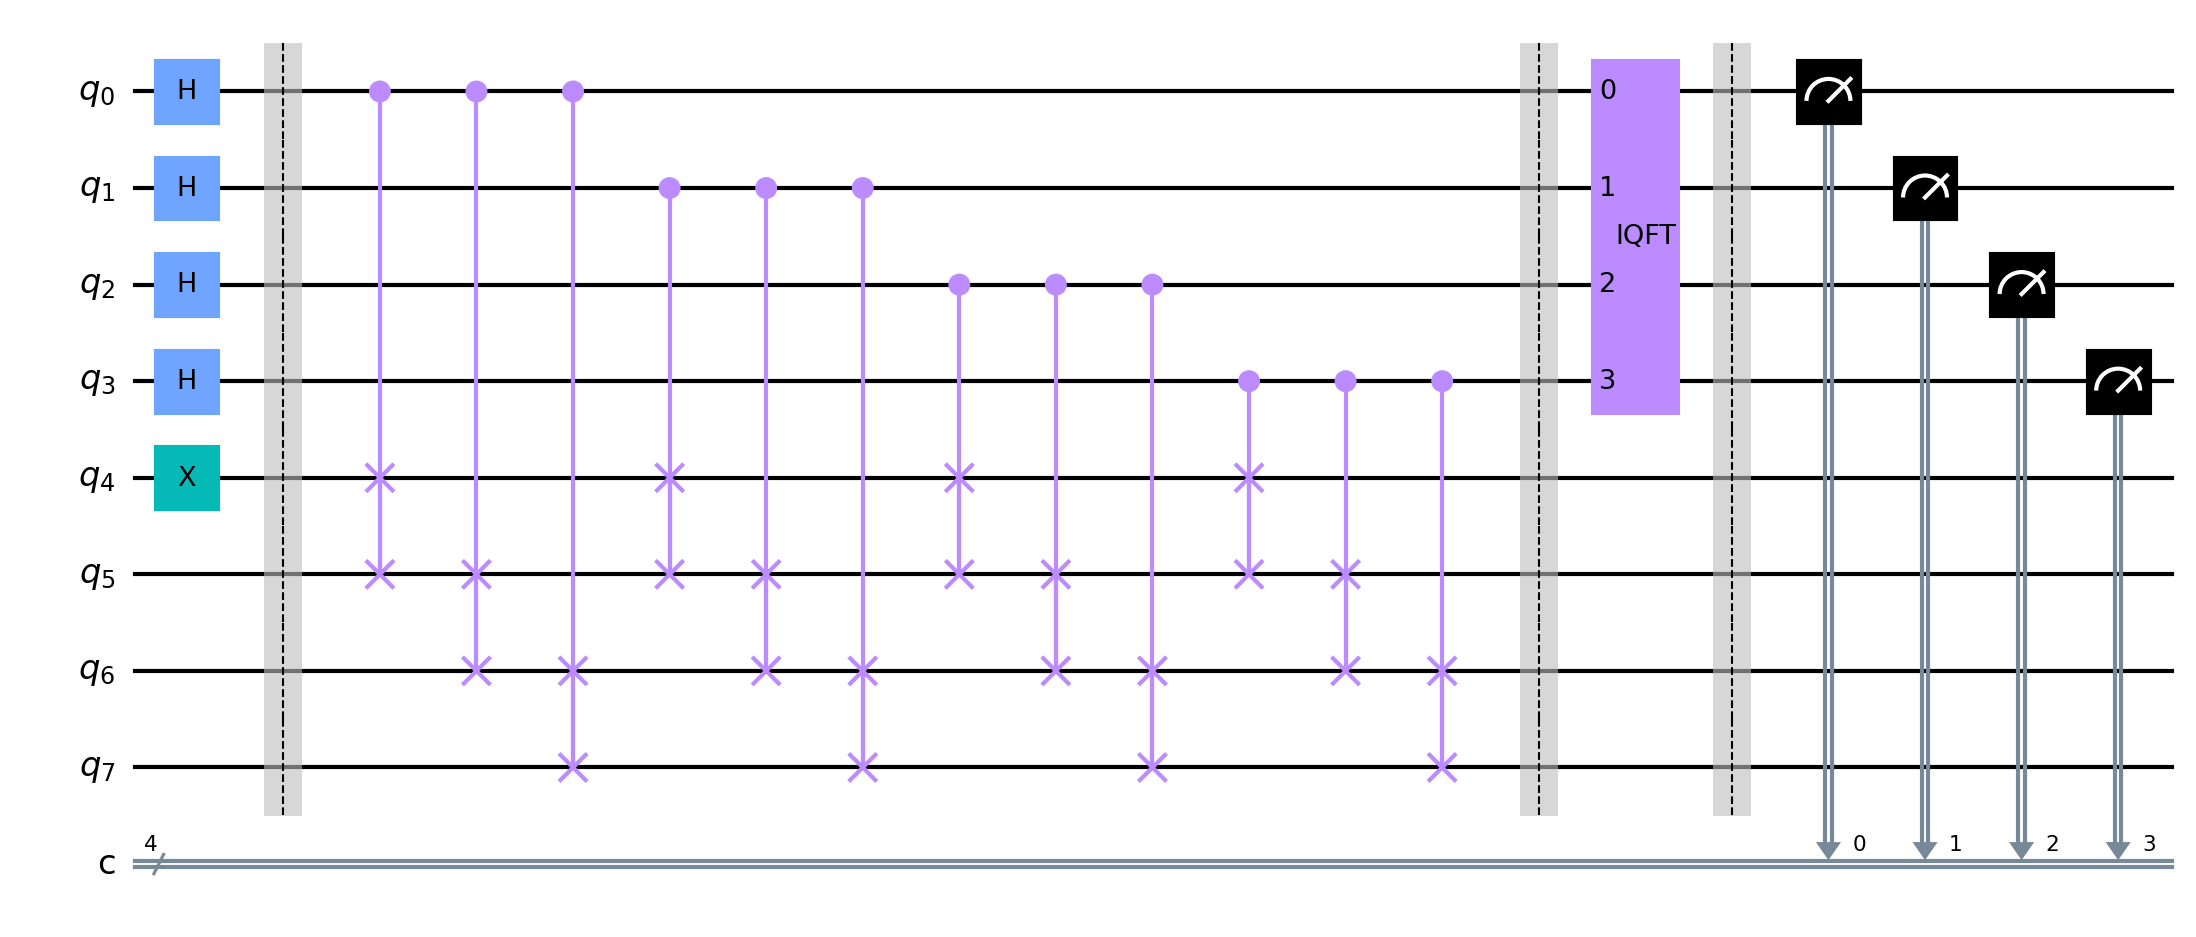
\includegraphics[width=\textwidth]{../media/images/shor_circuit.png}
    \caption{Quantum Circuit Representation of Shor's Algorithm}
    \label{fig:shor_circuit}
\end{figure}

\lstinputlisting[caption={Quantum Circuit for Shor's Algorithm (N=15, a=2)}]{../sims/shor_ckt.py}


\subsection{Time Complexity Analysis}

\begin{notebox}[title=Performance Comparison]
    The overall time complexity of Shor's Algorithm is:
    \[
        \mathcal{O}((\log N)^3)
    \]
    where $N$ is the integer to be factored. This is a polynomial-time complexity, representing an exponential speedup over the best-known classical factoring algorithms. For instance, the General Number Field Sieve (GNFS), a classical algorithm, has a sub-exponential time complexity of approximately:
    \[
        \mathcal{O}\left(e^{(\log N)^{1/3} (\log \log N)^{2/3}}\right)
    \]
    This stark contrast highlights the potential of quantum computing to solve certain problems much more efficiently than classical computing.
\end{notebox}

\section{Quantum Fixed-Point Attacks on RSA}

\begin{warningbox}[title=Alternative Threat Vector]
    Beyond Shor's algorithm, quantum computing introduces alternative methods to compromise RSA, such as fixed-point attacks. These attacks exploit the mathematical properties of RSA encryption to recover plaintext messages directly from ciphertexts without factoring the modulus \( n \).
\end{warningbox}

\paragraph{Fixed-Point Concept:} In RSA, a fixed point is a value \( M \) satisfying \( M^e \equiv M \mod n \). While such points are rare and typically not useful in classical cryptanalysis, quantum algorithms can efficiently identify these fixed points.

\paragraph{Quantum Algorithm Approach:} Researchers have proposed quantum algorithms that utilize quantum Fourier transforms to detect fixed points in RSA encryption. By preparing quantum superpositions and applying modular exponentiation, these algorithms can amplify the probability of measuring a fixed point, thereby recovering the original message \( M \) from the ciphertext \( C \) without needing to factor \( n \).

\paragraph{Implications:} Although these quantum fixed-point attacks are currently theoretical and require quantum computers with substantial capabilities, they highlight potential vulnerabilities in RSA that could be exploited as quantum technology advances. This underscores the importance of transitioning to quantum-resistant cryptographic schemes.


\section{Practical Limitations of Quantum Computing}

\begin{errorbox}[title=Current Challenges]
    Despite their potential, quantum computers face several significant practical challenges:

    \begin{enumerate}
        \item \textbf{Cost and Infrastructure:} Quantum systems are highly expensive to develop and maintain, requiring advanced infrastructure such as electromagnetic shielding and continuous monitoring. These demands currently restrict access to major corporations and research institutions.

        \item \textbf{Software, Tooling, and Talent Gaps:} Quantum software development remains at an early stage. Although frameworks like Qiskit are emerging, they lack mature toolchains and robust developer ecosystems. There is also a limited pool of talent with quantum computing expertise.

        \item \textbf{Hardware Limitations and Scalability:} Building quantum systems with large numbers of qubits is critical to solving meaningful problems. However, scaling introduces control complexity, increased noise, and greater cooling requirements.

        \item \textbf{Qubit Fragility and Decoherence:} Qubits must maintain delicate quantum states like superposition and entanglement, which are extremely sensitive to environmental disturbances such as temperature fluctuations and electromagnetic radiation. This leads to decoherence, one of the primary obstacles in practical quantum computation.
    \end{enumerate}
\end{errorbox}

\section{Post-Quantum Cryptography Alternatives}

\begin{successbox}[title=Future-Proof Solutions]
    \begin{itemize}
        \item \textbf{Lattice-Based:} CRYSTALS-KYBER, DILITHIUM, NTRU, Falcon.
        \item \textbf{Code-Based:} Classic McEliece.
        \item \textbf{Hash-Based Signatures:} SPHINCS+, XMSS, LMS.
        \item \textbf{Multivariate Polynomial:} Rainbow.
        \item \textbf{Isogeny-Based:} SIKE (broken), FrodoKEM.
    \end{itemize}
\end{successbox}

\newpage

\section{Conclusion}

\begin{infobox}[title=Summary of Findings]
    This report has explored the vulnerabilities of RSA encryption, particularly in the context of quantum computing threats. We've examined conventional weaknesses such as poor prime selection, where techniques like \textbf{Fermat's factorization} can efficiently break RSA when primes are too close together, and \textbf{Elliptic Curve Factorization} when one prime is significantly smaller than the other.

    The heart of our analysis focused on \textbf{quantum computing's ability to fundamentally undermine RSA's security guarantees}. Through an examination of quantum principles like superposition and the \textbf{Quantum Fourier Transform}, we demonstrated how \textbf{Shor's algorithm} provides an exponential speedup over classical factoring methods, reducing the time complexity from sub-exponential to polynomial \textbf{$\mathcal{O}((\log N)^3)$}. This efficiency makes it theoretically possible to break even large RSA keys in reasonable timeframes on sufficiently powerful quantum computers.

    While \textit{quantum fixed-point attacks} offer alternative methods to compromise RSA encryption, significant practical challenges remain in quantum computing implementation:

    \begin{itemize}
        \item \textbf{Prohibitive costs and infrastructure requirements}
        \item \textbf{Qubit fragility and decoherence}
        \item \textbf{Lack of mature software development toolchains}
    \end{itemize}

    The imminent threat to RSA has accelerated research into \textbf{post-quantum cryptographic alternatives}, with various approaches including:

    \begin{center}
        \begin{tabular}{|c|c|c|}
            \hline
            \rowcolor{gray!20} \textbf{Lattice-Based} & \textbf{Code-Based} & \textbf{Hash-Based} \\
            \hline
            CRYSTALS-KYBER                            & Classic McEliece    & SPHINCS+            \\
            DILITHIUM                                 &                     & XMSS                \\
            NTRU                                      &                     & LMS                 \\
            \hline
        \end{tabular}
    \end{center}

    Organizations like \textbf{NIST} are actively standardizing these new methods to ensure data security in a post-quantum world.

    As quantum computing technology advances, the transition to \textbf{quantum-resistant cryptographic systems} becomes increasingly urgent. The future of secure communication will likely involve a hybrid approach during the transition period, ultimately leading to widespread adoption of post-quantum cryptographic standards that can withstand attacks from both classical and quantum adversaries.
\end{infobox}

\newpage
\section{Acknowledgements}

We sincerely thank \textbf{Dr. Krishna Mohan Parattu} Sir for providing us with this valuable opportunity. We also acknowledge \textbf{Dr. Awaneesh Kumar Yadav} Sir and his course, Information Security and Privacy, for enriching our understanding of cryptography. Their guidance and encouragement were instrumental in shaping this project.

We are grateful to \textbf{Anthropic} for offering the tools and resources that supported our development process.

We extend our appreciation to open source resources like Qiskit, NumPy, and educational YouTube channels, especially \textbf{3Blue1Brown} and \textbf{Veritasium}, which have been invaluable in helping us visualize and understand complex mathematical concepts.

Lastly, we deeply appreciate our parents and peers for their constant support and motivation throughout this journey.

\newpage
\section{References}

\begin{enumerate}
    \item 3Blue1Brown. (2018). "But what is the Fourier Transform? A visual introduction." [Video]. YouTube.
          \url{https://youtu.be/spUNpyF58BY}

    \item Veritasium. (2023). "How Quantum Computers Break The Internet... Starting Now" [Video]. YouTube.
          \url{https://www.youtube.com/watch?v=-UrdExQW0cs}

    \item minutephysics. (2019). "How Quantum Computers Break Encryption | Shor's Algorithm Explained" [Video]. YouTube.
          \url{https://youtu.be/lvTqbM5Dq4Q}

    \item Paar, Christof, and Jan Pelzl. \textit{Understanding Cryptography: A Textbook for Students and Practitioners}. Springer, 2009.

    \item Obregon, A. (2023). "A Beginner's Guide to Quantum Computing Fundamentals." Medium.
          \url{https://medium.com/@AlexanderObregon/a-beginners-guide-to-quantum-computing-fundamentals-c11de9187892}

    \item Wikipedia contributors. (2023). "Quantum Fourier transform." Wikipedia, The Free Encyclopedia.
          \url{https://en.wikipedia.org/wiki/Quantum_Fourier_transform}

    \item Wikipedia contributors. (2023). "Qubit." Wikipedia, The Free Encyclopedia.
          \url{https://en.wikipedia.org/wiki/Qubit}

    \item PhysicsWorks. (2018). "Quantum Fourier Transform." PhysicsWorks.
          \url{https://physicsworks2.com/quantum%20information%20and%20computation/2018/05/02/quantum-fourier-transform.html}

    \item Post-Quantum. (2023). "Shor's Algorithm: A Quantum Threat." Post-Quantum.
          \url{https://postquantum.com/post-quantum/shors-algorithm-a-quantum-threat/}

    \item Quantum Zeitgeist. (2023). "Beyond the Hype: Understanding the Limitations of Quantum Tech." Quantum Zeitgeist.
          \url{https://quantumzeitgeist.com/beyond-the-hype-understanding-the-limitations-of-quantum-tech/}
\end{enumerate}

\newpage
\section{Roles and Responsibilities}
This project was completed through collaborative effort, with each team member making significant contributions in various capacities. The table below outlines the specific roles and responsibilities undertaken by each member of the team.

\begin{center}
    \begin{tabularx}{\textwidth}{|l|X|c|c|c|}
        \hline
        \rowcolor{gray!20} \textbf{Team Member} & \textbf{Research Topics}                                                    & \textbf{PPT} & \textbf{Report} & \textbf{Simulations} \\
        \hline
        \textbf{Jigar Fufal}                    & RSA fundamentals and weaknesses, Post-quantum cryptographic alternatives    & \checkmark   & \checkmark      &                      \\
        \hline
        \textbf{Ojas More}                      & Elliptic Curve Factorization, Fized Point Attacks on RSA                    &              & \checkmark      &                      \\
        \hline
        \textbf{Parth Gawande}                  & Fourier Transform and Wrapping theory, Fermat's Factorization Theorem       &              & \checkmark      &                      \\
        \hline
        \textbf{Abhishek Mantri}                & Practical limitations of quantum computing                                  & \checkmark   & \checkmark      &                      \\
        \hline
        \textbf{Arani Ghosh}                    & Quantum Fourier Transform (QFT) and its application in Shor's Algorithm     & \checkmark   & \checkmark      &                      \\
        \hline
        \textbf{Arka Mukhopadhay}               & Introduction to quantum computing, qubit theory, quantum measurement theory &              & \checkmark      & \checkmark           \\
        \hline
        \textbf{Harshit Jain}                   & Shor's Algorithm, Quantum Gates and Qubits                                  & \checkmark   & \checkmark      & \checkmark           \\
        \hline
    \end{tabularx}
\end{center}


\end{document}